\documentclass[twocolumn,10pt]{article}

\usepackage[utf8]{inputenc}
\usepackage{amsmath}
\usepackage{amssymb}
\usepackage{amsthm}
\usepackage{graphicx}
\usepackage{times}
\usepackage{geometry}
\usepackage[ruled,vlined]{algorithm2e}

\usepackage[switch]{lineno}
\linenumbers

\newtheorem{definition}{Definition}
\newtheorem{property}{Property}
\newtheorem{claim}{Claim}

\DeclareMathOperator{\unif}{unif}
\DeclareMathOperator{\sample}{sample}
\DeclareMathOperator{\setcount}{count}
\DeclareMathOperator{\mode}{mode}
\DeclareMathOperator*{\argmax}{arg\,max}
\DeclareMathOperator*{\argmin}{arg\,min}

\usepackage{geometry}
\geometry{left=1.5cm,right=1.5cm,top=2cm,bottom=2cm}
\setlength{\columnsep}{0.5cm}

\title{Supplementary Information: \\
Small interlocking groups improve mass deliberation\\in the presence of strong social influence}
\author{
%Edward L. Platt\\
%University of Michigan\\
%elplatt@umich.edu
%and
%Herminio Bodon\\
%Northwestern University\\
%HerminioBodon2020\\@u.northwestern.edu
%\and
%Daniel M. Romero\\
%University of Michigan\\
%drom@umich.edu
Authors Redacted \\
for \\
Double-Blind Peer-Review
}
\date{\today}

\begin{document}

\maketitle

\section{Simulation Procedure}
We begin with a network $(V,E_t)$. The vertices $V$ correspond to agents. The edges $E_t$ allow agents to exchange information with their immediate neighbors at time $t$.
Agents collaborate to find a solution $s$ from a space of solutions $\mathcal{S}$ that maximizes an objective function $Q(s)$.
We use binary strings of length $d$ as our solution space: $s \in \mathbb{Z}^d$.
At any one time $t$, each agent $v$ has exactly one preferred solution $s_{v,t}$.
We generate a tunably rugged objective function $Q(s)$ using an NK-Model \cite{kauffman_towards_1987} (see Section \ref{subsec:task}) with N=15, K=6, exp=8.

The simulation begins at time $t=0$ by generating a set of initial solutions $s_{v,0}$ for the agents. These are generated randomly, with each possible solution having equal probability.
The simulation proceeds iteratively.
At time $t$ each agent applies one of several {\em learning strategies} (see Section \ref{sec:learning}), to determine its preferred solution at time $t+1$.
Learning strategies can rely on the agent's own solution, the solutions of its neighbors, and potentially additional information shared by its neighbors.
Learning strategies may also incorporate information about the objective function, modeling an agents' ability to evaluate the quality of solutions (see Section \ref{sec:capability}).
To allow for ties, learning strategies produce a set of solutions rather than a single solution.
In our simulations, we choose winners at random in the case of a tie.
We allow the simulation to proceed for 300 iterations, which we have found sufficient to guarantee convergence with our chosen parameters.

\section{Network Topologies}

We use networks to represent constraints on who talks to whom. Each agent is represented by a vertex, and two agents are able to interact when their vertices are connected by an edge. In this paper we are concerned with network deliberation, which takes place on interlock networks. Interlocks are composed of small cliques (i.e., pods) with some vertices belonging to multiple cliques. For the interlock networks in this paper, each vertex belongs to exactly one pod at a time, with pod membership periodically reassigned to achieve multiple membership. As a control, we also consider networks representing conventional deliberation.

\subsection{Conventional Deliberation}
We model the communication network structure of conventional deliberation using two static networks: small-world networks \cite{watts_collective_1998}, and preferential attachment networks \cite{barabasi_emergence_1999}. In typical deliberative settings, from deliberative assemblies to online forum threads, the contributions of any member are potentially visible to all other members.
The network of {\em potential} communication can be modelled by a complete graph.
However, a complete graph may not be the best model for the {\em actual} communication that takes place in such a network. In a real-world deliberation, some participants are more influential than others \cite{goel_structure_2012, shaw_laboratories_2014}, and many communications can be missed or ignored by any particular participant.

Human social networks often exhibit large clustering, and short path lengths.
To model such dynamics, we use Watts-Strogatz small-world networks  \cite{watts_collective_1998}.
These networks model, for example, when participants interact mostly with their strong ties, but occasionally with a weak tie. Social networks have also been found to exhibit skewed degree distributions with long tails \cite{barabasi_emergence_1999}.
We model these networks using the Barabási-Albert preferential attachment model.
These networks model settings where a small number of individuals produce a disproportionate share of the communication due to factors such as social capital, expertise, or confidence.

\subsection{Network Deliberation: Interlock Networks}
Both of our network deliberation conditions use networks built from interlocking pods.
These pods are small complete graphs of roughly equal size.
At any given time, each agent can communicate with all other agents in exactly one pod.
Periodically, all agents are simultaneously reassigned to new pods.
These reassignments create an interlocking structure, allowing information to flow through the entire group.
This structure can be represented as a time-dependent or directed network.
The properties of an interlock network depend on the particular method for assigning agents to pods.
Crucially, interlocking structure is created when agents are placed with others they have not yet interacted with.
We thus require that pod assignment schemes satisfy the following mixing property:
\begin{property}
\label{prop:mixing}
For any agent $v$, and any two assignment stages $t$, $t^\prime$, the probability that at least one neighbor of $v$ at stage $t$ is also a neighbor at stage $t^\prime$ approaches 0 as $|V|$ grows.
\end{property}

\subsubsection{Random-Pod Assignment}
The {\em random-pod} assignment method (Algorithm \ref{alg:random}) simply assigns agents to groups at random. Pseudocode for this method is shown in Algorithm \ref{alg:random}.

\begin{algorithm}
\SetAlgoLined
\DontPrintSemicolon
\SetKwFunction{removeRandom}{removeRandom}
\SetKwFunction{insert}{insert}
\SetKwFunction{emp}{empty}
\SetKw{algnot}{not}
\KwData{A vertex list $V$, the pod size $M \in \mathbb{Z}$.}
\KwResult{A partition of the vertices.}
    $N \longleftarrow \lceil \frac{|V|}{M} \rceil$ \;
    $P \longleftarrow$ List of $N$ empty sets \;
    \For{$i \in 1, \ldots, M$}{
        \ForEach{$s \in P$}{
            \If{\algnot $V.\emp()$}{
                $v \longleftarrow V.\removeRandom()$ \;
                $s.\insert(v)$ \;
            }
        }
    }
    \Return{$P$}
\caption{Random-Pod Assignment}
\label{alg:random}
\end{algorithm}

\begin{claim}
Random-pod assignment satisfies Property \ref{prop:mixing}.
\end{claim}

\begin{proof}
Let $v$ be a vertex of graph $G=(V,E_t)$ with a set of $M$ neighbors at stage $t$ denoted $N_t(v)$.
The probability that the $k$th neighbor chosen at time $t^\prime \neq t$ belongs to $N_t(v)$, given that the first $k - 1$ did not, is:
\begin{align*}
p_\text{repeat}(k)
&= \frac{M - 1}{|V| - k} \\
&\leq \frac{M - 1}{|V| - M}.
\end{align*}
The probability that none of the $M-1$ neighbors chosen at time $t^\prime$ belong to $N(v)$ thus satisfies:
\begin{align*}
p_\text{mixed}
&\geq
\left( 1 - \frac{M - 1}{|V| - M} \right)^{M-1} \\
\lim_{|V|\rightarrow\infty} p_\text{mixed}
&= 1
&\qedhere
\end{align*}
\end{proof}

Random pod assignment also creates structurally efficient networks with short geodesic distances, as shown in Figure \ref{fig:broadcast}.
There has been evidence both for
\cite{lazer_network_2007, derex_partial_2016, mason_propagation_2008, barkoczi_social_2016}
and against
\cite{mason_collaborative_2012, barkoczi_social_2016}
the effectiveness of structurally efficient networks in social learning.

\begin{figure}
    \centering
    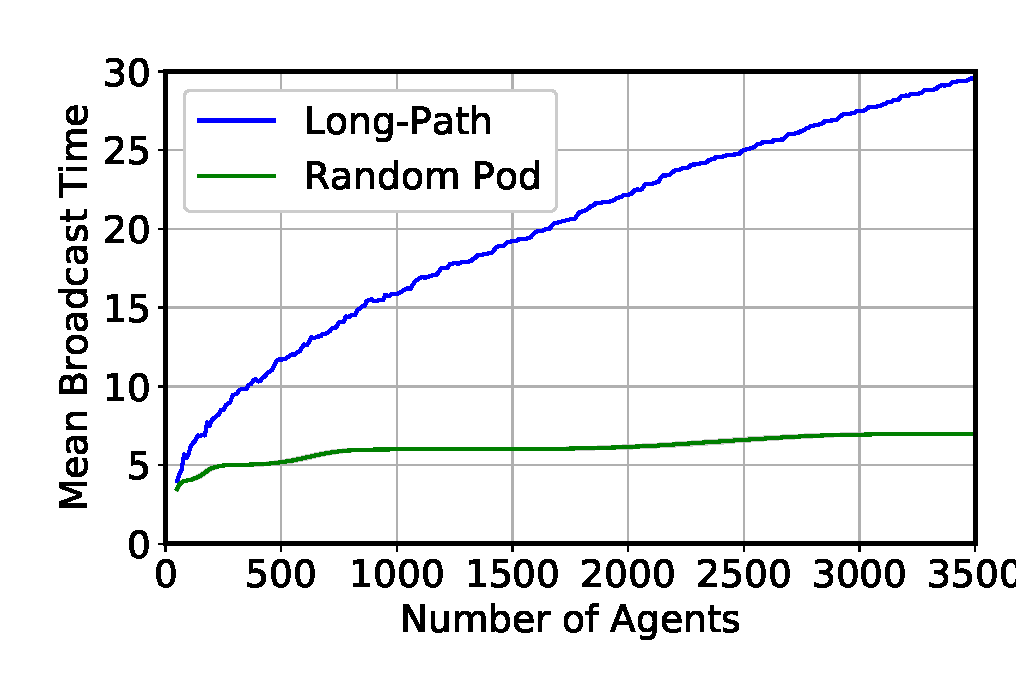
\includegraphics[width=3.33in]{fig-broadcast.eps}
    \caption{Mean time necessary for a signal broadcast from one node to reach the entire network. We use mean broadcast time is used as a measure of geodesic length for time-varying networks.}
    \label{fig:broadcast}
\end{figure}


\subsubsection{Long-Path Pod Assignment}

To study the effects of path length, we require an alternative pod assignment method that produces long paths.
However, we must still retain Property \ref{prop:mixing} such that it is rare for two agents to repeatedly share the same pod.
This property ensures the creation of many new edges at each stage, which is difficult--but not impossible--to reconcile with long average path length.
We now present a {\em long-path} pod assignment method, which meets both of the above goals.

We begin with a high-level overview.
Agents are assigned an integer position on a 1-dimensional circular lattice.
By preferring short-distance links on this lattice, we maintain long path lengths.
We also partition agents according to the remainder of their position, modulo some prime, i.e., their residue class.
By limiting links to agents in the same residue class, and using a unique prime at each stage, we ensure that it is rare for multiple agents to share a pod twice in a row.
Specifically, for stages using primes $p$ and $q$, two agents will share a pod for both stages when their positions are equal modulo $pq$. Pseudocode for long-path assignment is shown in Algorithm \ref{alg:long}.

\begin{algorithm}
\SetAlgoLined
\DontPrintSemicolon
\SetKw{algnot}{not}
\SetKwFunction{removeRandom}{removeRandom}
\SetKwFunction{moduli}{moduli}
\SetKwFunction{append}{append}
\SetKwFunction{enqueue}{enqueue}
\SetKwFunction{dequeue}{dequeue}
\SetKwFunction{concat}{concatenate}
\KwData{A vertex list $V$, the pod size $M \in \mathbb{Z}$, the stage $t \geq 0 \in \mathbb{Z}$, a list of co-prime integers $\moduli$.}
\KwResult{A partition of the vertices.}
    $N \longleftarrow \lceil \frac{|V|}{M} \rceil$ \;
    $P \longleftarrow$ List of $N$ empty sets \;
    \eIf{$t = 0$}{
        // Place all vertices in same residue class \;
        $p \longleftarrow 1$ \;
    }{
        // Choose integer to define residue class \;
        $p \longleftarrow \moduli[t]$ \;
    }
    // Assign vertices to residue classes \;
    $R \longleftarrow$ List of $p$ empty queues \;     
    \For{$z \in 0, \ldots, |V|-1$}{
        $R[z \bmod p].\enqueue(V[z])$ \;
    }
    // Divide each residue class into pods \;
    $P \longleftarrow $ Empty list of lists. \;
    \For{$r \in R$}{
        $N_r \longleftarrow \lceil \frac{|r|}{M} \rceil$ \;
        $P_r \longleftarrow$ List of $N_r$ empty lists \;
        \For{$i \in 1, \ldots, M$}{
            \For {$j \in 0, \ldots, N_r - 1$}{
                \If{ \algnot $r.\emp()$}{
                    $v \leftarrow r.\dequeue()$ \;
                    $P_r[j].\append(v)$ \;
                }
            }
        }
        $P.\concat(P_r)$
    }
    \Return{$P$}
\caption{Long-Path Assignment}
\label{alg:long}
\end{algorithm}


\begin{claim}
When the pod size $M$ is less than the modulus $p_t$ for all stages $t$, long-path pod assignment satisfies Property \ref{prop:mixing}.
\end{claim}

\begin{proof}
Let $p$ and $q$ be co-prime integers used as moduli for stages $t$ and $t^\prime$ respectively.
Let $z(x)$ denote the integer position of vertex $x$.
Let $v$ be a vertex, and let us assume vertex $w$ belongs to the same pod as $v$ at both time $t$ and $t^\prime$.
This assumption implies:
\begin{align*}
    z(v) &\equiv z(w) \pmod{p} \\
    z(v) &\equiv z(w) \pmod{q} \\
    \implies z(v) - z(w) &\equiv 0 \pmod{p} \\
    &\equiv 0 \pmod{q} \\
    &= npq & \text{for some integer n}.
\end{align*}
By the definition of the long-path algorithm:
\begin{align*}
    |z(v)-z(w)| & \leq (M - 1)p \\
    \implies |n|pq & \leq (M - 1)p \\
    |n|q & \leq (M - 1).
\end{align*}
By assumption, $q \geq M$, so the above can only be satisfied by $n=0$,
which in turn implies $v=w$. \qedhere
\end{proof}

To see that the long-path procedure produces long geodesics, note that the pods of size $M$ connect nodes at most $(M - 1)p_i$ apart in position, preventing the creation of any shortcut edges, as long as $p_i$ is small compared to $|V|$.
Numerical simulations confirm that the long-path algorithm produces geodesics larger than random pod assignment (Figure \ref{fig:broadcast}).
The number of agents may not be an exact multiple of $M$, so the final pods may be truncated. However, the network will be a sub-graph of a network that does have a multiple of $M$ nodes, so the structure will not be fundamentally changed, and these edge effects should become negligible as the number of agents increases.

\section{Learning Strategies}
\label{sec:learning}
The choice of network structure defines which agents can exchange information, but not how those agents act on the information received. An agent's actions based on available information are determined by that agent's {\em learning strategy}. Learning strategies can be divided into {\em individual learning strategies} which use only information directly observable by the agent, and {\em social learning strategies} which use information communicated by neighboring agents.

Generally, a learning strategy may incorporate both social and individual components, but we will discus each individually before approaching hybrid strategies. The learning strategies available to an agent also depend on the agent's ability to evaluate the quality of candidate solutions, which we refer to as its {\em capabilities}, which we now explore in further detail.


\subsection{Agent Capabilities}
\label{sec:capability}
In human social learning, the ability of individuals to evaluate the quality of a solution can vary with factors such as expertise and task type. When comparing learning strategies, it will be helpful to classify them according to the capabilities they require of agents. We formalize these capabilities as oracle functions, which accept one or more task solutions as input and reveal whether the supplied state(s) satisfy some particular property.

One of the strongest capabilities an agent might posses, is to compare two arbitrary solutions to determine which yields a higher value of the objective function. We represent this capability using the {\em arbitrary comparison} oracle.
\begin{definition}
The arbitrary comparison oracle $\mathcal{O^>}(s_1, s_2)$ is given by:
\begin{eqnarray}
\mathcal{O}^>(s_1, s_2) &\equiv&
Q(s_1) > Q(s_2)
\end{eqnarray}
\end{definition}

Under a weaker assumption, agents might be ``experts'' on their current solution and able to compare that particular solution to any other. This ability is represented by a {\em single-solution comparison} oracle.
\begin{definition}
The single-solution comparison oracle for solution $s$ is given by:
\begin{eqnarray}
\mathcal{O}^>_s(\tilde{s}) &\equiv&
Q(\tilde{s}) > Q(s)
\end{eqnarray}
\end{definition}

In many contexts, it is reasonable to assume that agents can explore the effects of small changes to their current solution. When the solutions are binary strings, such variations can be modeled by flipping a single bit of the solution string. We formalize this capability through the {\em mutation comparison} oracle.
\begin{definition}
The mutation comparison oracle for solution $s$ is given by:
\begin{eqnarray}
\mathcal{O}^\oplus_s(i) &\equiv&
Q(s \oplus e_i) > Q(s),
\end{eqnarray}
where $\oplus$ represents addition mod 2 and $e_i$ represents the binary string with a single 1 at index $i$.
\end{definition}

\subsection{Mutation-Based Individual Learning}
In real-world collaborations, individuals sometimes work independently, even when communication is available. Independent work might be motivated by practical concerns (such as distributing labor) or by social dynamics. We model individual learning using single-bit mutations, following the examples of
\cite{lazer_network_2007} and \cite{barkoczi_social_2016}. Agents constructs a candidate solution by flipping a single bit of their solution at an index selected uniformly at random. If the candidate solution yields a higher value of the objective function, the agent adopts it as the new solution. As this strategy requires comparing solutions that differ by at most one bit, an oracle at least as powerful as the mutation comparison oracle is required.

\begin{definition}
The mutation individual learning strategy $\mathcal{L}_{\text{I}}(v)$ is defined as:
\begin{eqnarray}
i &\sim& \unif(1,d) \nonumber\\
\mathcal{L}_{\text{I}}(v) &\equiv&
\begin{cases}
\{s(v) \oplus e_i\} & \mbox{if $\mathcal{O}^{\oplus}_{s(v)}(i)$}
\\
\{s(v)\} & \mbox{otherwise}.
\end{cases}
\end{eqnarray}
\end{definition}

\subsection{Best-Neighbor}
Among social strategies, the straightforward greedy approach results in the {\em best-neighbor} strategy, which has been widely used in prior work \cite{lazer_network_2007, mason_propagation_2008, barkoczi_social_2016}. In this strategy, an agent simply compares the solutions of all agents in its neighborhood and adopts the best. While straightforward, this strategy makes a strong assumption about agent capabilities: access to the arbitrary comparisons.
\begin{definition}
The Best-Neighbor strategy $\mathcal{L}_{BN}(v)$ is defined as:
\begin{eqnarray}
\mathcal{L}_{BN}(v)
&\equiv&
\{ \, s \!\in\! S(v)
\mid
\forall \tilde{s} \!\in\! S(v) \, \
\lnot \, \mathcal{O}^{>}(\tilde{s}, s),
\end{eqnarray}
where $S(v)$ is the multiset of solutions of $v$'s neighbors.
\end{definition}

\subsection{Confident-Neighbor}
This paper introduces {\em confident-neighbor}, an alternative to the best-neighbor strategy which relies only on the single comparison oracle and which reduces to best-neighbor for interlocking pod networks. The confident neighbor strategy also represents a moderate level of social loafing \cite{karau_social_1993}, in which agents do not actively seek to improve their solution, but passively adopt better solutions if they are presented.

Confident neighbor proceeds in two stages. In the first stage, agents determine if their current solution is at least as good as all others in their neighborhood. If so, we call the agent {\em confident}. In the second stage, confident agents broadcast their solution to all of their neighbors. Non-confident agents choose randomly between any broadcast solutions they receive, or keep their original solution if they receive none.

\begin{definition}
The confident-neighbor strategy $\mathcal{L}_{CN}$ is defined as:
\begin{eqnarray}
C(v) &\equiv& \{
\, s(w)  \nonumber \\
&& \,
\mid
\forall w \!\in\! N(v) \, \forall u \!\in\! N(w) \,
\lnot \, \mathcal{O}^{>}_{s(w)}(s(u)) \,
\}
\\
\mathcal{L}_{\text{CN}}(v)
&\equiv& 
\begin{cases}
C(v) & \text{if } C(v) \neq \varnothing \\
\{ \, s(v) \, \}& \text{otherwise,}
\end{cases}
\end{eqnarray}
where $N(v)$ is the set of vertices neighboring $v$ and $s(v)$ is the current candidate solution for agent $v$.
\end{definition}

Confident-neighbor differs from best-neighbor because of two subtle but important considerations. First, an agent's neighbors need not be adjacent to each other. Second, an agent's neighbors can be adjacent to others outside that agent's neighborhood. As a result, an agent might receive zero, one, or many broadcasts. The exception is when agents belong to a clique (e.g., in network deliberation), in which case agents receive exactly one broadcast for each maximal solution in the clique, thus yielding the same results as best-neighbor. Confident-neighbor is thus more appropriate than best-neighbor for comparing network deliberation to single group deliberation, as the same information is utilized in both cases.


\subsection{Conform}
In some contexts, agents might rely on information other than solution quality in their learning strategies.
Agents might do so out of necessity if they are not able to compare arbitrary solutions.
Alternatively, agents might ignore solution quality due to social dynamics, e.g. social loafing \cite{karau_social_1993}. In these contexts, agents might instead evaluate solutions based on popularity, which produces the {\em conform} learning strategy.
When using the conform strategy, agents count the number of times each solution appears among their neighbors, and adopt the most popular.
\begin{definition}
The conform strategy $\mathcal{L}_{\text{C}}(v)$ is defined as:
\begin{eqnarray}
\mathcal{L}_{\text{C}}(v) &=&
\mode(S(v)),
\end{eqnarray}
where $S(v)$ is the multiset of candidate solutions for all vertices neighboring $v$, and $\mode()$ returns a set containing the mode or modes of a multiset.
\end{definition}
Note that the conform strategy does not depend on the objective function or any oracles, meaning it incorporates no new information about the quality of the solutions.

% Exclude bitwise majority from paper
\iffalse

\subsection{Bitwise Majority}
Instead of evaluating entire solutions on their popularity, it is also possible to evaluate the popularity of each component of a solution, i.e., each bit in the bit string \cite{platt_network_2018}.
We refer to this strategy as {\em bitwise majority} social learning.
As with previous strategies, bitwise majority can result in ties for individual bits, which result in ties for the resulting full solution.

\begin{definition}
The bitwise majority strategy $\mathcal{L}_{bitwise}$ is defined as:
\begin{eqnarray}
S_i &=& \bigcup_{x \in S} \{x_i\} \\
\mathcal{L}_{bitwise}(S)
&=& \mode(S_1) \times \mode(S_2) \ldots \times \mode(S_d),
\end{eqnarray}
where $x_i$ is the $i$th element of the binary string $x$,
$S_i$ is a multiset, and $\mode(S)$ returns a set containing the mode or modes of $S$, and $\times$ is the Cartesian product.
\end{definition}
As with conform, the bitwise majority strategy does not incorporate any new information about solution quality.
Bitwise majority also has the notable property of being able to produce novel solutions that vary significantly from any previously seen.

% End of bitwise majority
\fi

\subsection{Combining Learning Strategies}\label{subsubsec:combine}
Models of social learning often combine truly social strategies with individual learning \cite{lazer_network_2007, barkoczi_social_2016,gomez_clustering_2019}.
We find that the method used to combine social and individual strategies can result in a notable difference in outcome. As a robustness check, we consider two cases for all of our analyses:
\begin{description}
\iffalse
\item[Serial]{
Agents first perform individual learning to produce an intermediate solution, and then apply social learning to the intermediate solutions. This method does not rely on any of the solution comparison oracles.}
\fi
\item[Parallel]{
Agents apply both social and individual learning strategies to their initial solution to produce two competing intermediate solutions, then adopt the better of the two. This method relies on the arbitrary comparison oracle.}
\item[Fallback]{
Agents first apply social learning to the current solution, but "fall back" to individual learning if the result is not an improvement on the original solution \cite{lazer_network_2007, barkoczi_social_2016,gomez_clustering_2019}. Fallback relies on the single comparison oracle and could be motivated by limited agent capability or social loafing.}
\end{description}

\iffalse
We must also consider {\em criticality} \cite{barkoczi_social_2016, rendell_rogersparadox_2010}.
After combining individual and social learning according to one of the above methods, non-critical agents immediately adopt the result.
Critical agents, on the other hand, compare the quality of the new solution to their previous solution, only adopting the new one if it provides an improvement.
Note that critical behavior relies on information about solution quality and requires single-solution comparison capability, or stronger.
\fi


\section{NK Model}
\label{subsec:task}
The NK Model \cite{kauffman_towards_1987} is an optimization problem particularly well-suited for modelling complex tasks. The model is used to create a fitness function $Q(s)$ over some discrete space $\mathcal{S}$, typically binary strings of a fixed length.
The model is parameterized by two variables.
The first, $N$, is the dimension of the solution space, i.e., the length of each binary string.
The second parameter, $K$, determines the ``ruggedness'' of the fitness function, i.e., the number of local maxima.
In effect, the $K$ parameter allows the complexity of the optimization problem to be tuned.
The ability to tune task complexity makes the NK model well-suited for studying the role of complexity in various settings.
The construction of an NK fitness function from a set of parameters is a stochastic process.
So particular values of $N$ and $K$ define a class of fitness functions, which can be sampled to produce a specific fitness function.

We now show the construction of the NK model fitness function.
A class of NK model fitness functions can be defined by a tuple of integer parameters
$(N, K)$ such that $N > 0$ and $0 \leq K < N$.
We begin by defining $N$ fitness contributions functions:
\begin{eqnarray}
q_i &:& \mathbb{Z}^{K+1} \rightarrow [0, 1].
\end{eqnarray}
The value of each $q_i(x)$ is chosen uniformly at random in the range $[0, 1]$ at the time the function is defined.
We also define $N$ projection operators $P_i$ which select $K+1$ bits from a length-$N$ bit string.
Each $P_i$ selects the bit at index $i$ and $K$ other indices, chosen uniformly at random at the time $P_i$ is constructed.
For a solution $s$, the $i$th fitness contribution is evaluated on the $K + 1$ bits selected by the $i$th projection: $q_i(P_i(s))$.
The value of the fitness function is the mean of all fitness contributions:
\begin{eqnarray}
Q(s) &=& \frac{1}{N}\sum_{i=1}^N q_i(P_i(s)).
\end{eqnarray}

The parameter $K$ alters the ruggedness of the fitness function by controlling the interdependence between the $q_i$.
When $K = 0$, each $q_i$ depends on a single unique index of $s$,
allowing the $q_i$ to be optimized independently.
In this case, $Q(s)$ has a single maximum: the global maximum.
However, for $K > 0$, two things happen: it becomes possible for each $q_i$ to have multiple local maxima, and some of the $q_i$ become coupled due to dependence on the same indices of $s$.
The result is that as $K$ increases, both the number of local maxima of $Q(s)$ \cite{weinberger_local_1991} and the difficulty of simultaneously optimizing the $q_i$ increase.
In other words, $Q$ becomes more rugged, and more complex.

The distribution of local maximum values is asymptotically normal for large $K$ \cite{weinberger_local_1991}.
When a skewed distribution is preferred, it is common to exponentiate the value of $Q(s)$ as a final step \cite{lazer_network_2007, barkoczi_social_2016, gomez_clustering_2019}.

\section{Supplemental Results}

Figures \ref{fig:results-frac-parallel} and \ref{fig:results-frac-fallback} show pairwise comparisons of solution quality between strategy/network settings. Figures \ref{fig:results-bn-parallel-dist}--\ref{fig:results-conf-fallback-dist} show the complete solution quality distributions for all settings.
Tables \ref{tab:t-instrat-fallback}--\ref{tab:t-innet-parallel} show the t-values and Bonferroni-corrected p-values for comparisons across networks and strategies.

\begin{figure}
    \label{fig:results-frac-parallel}
    \centering
    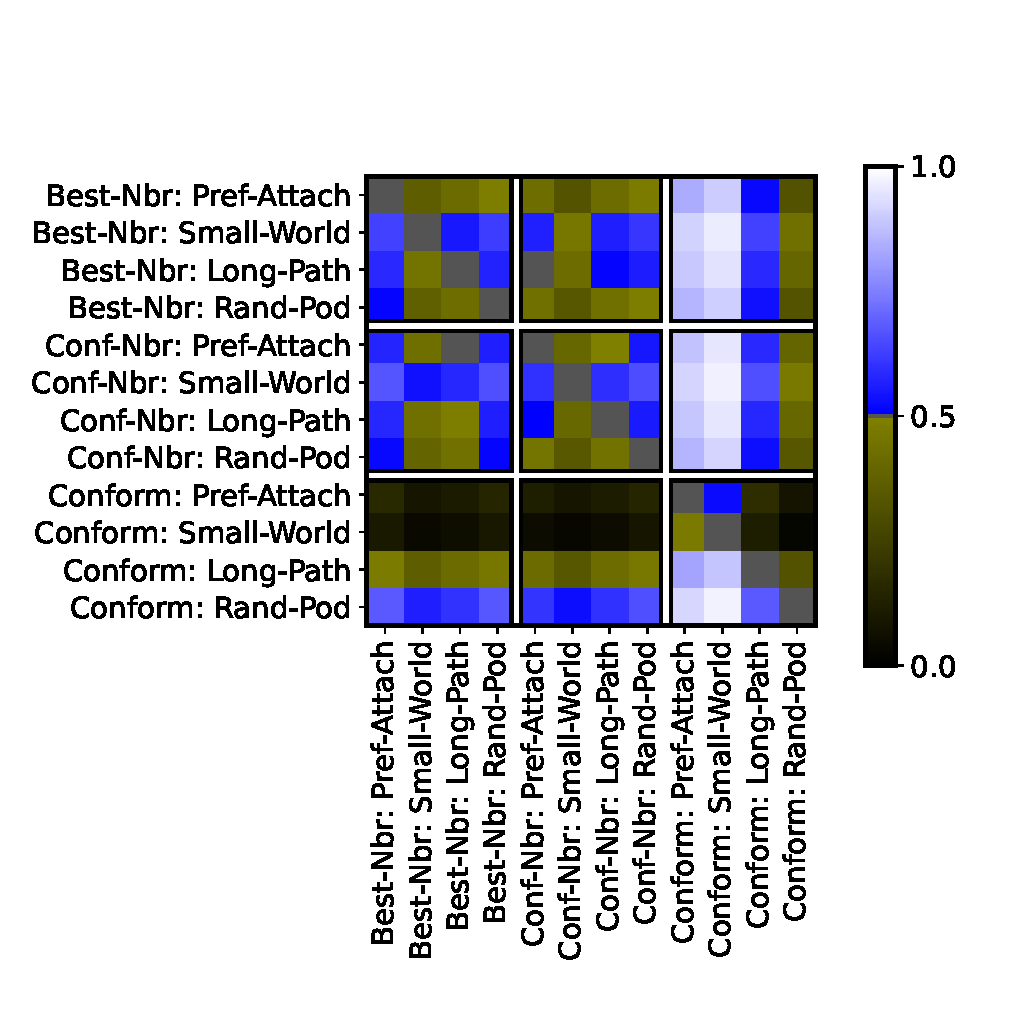
\includegraphics[width=3.33in]{fig-result-frac-parallel.eps}
\caption{Fraction of simulations in which the row condition outperforms the column condition. Results are shown for parallel individual learning. In the case of a tie, weight is divided evenly.}
\end{figure}

\begin{figure}
    \label{fig:results-frac-fallback}
    \centering
    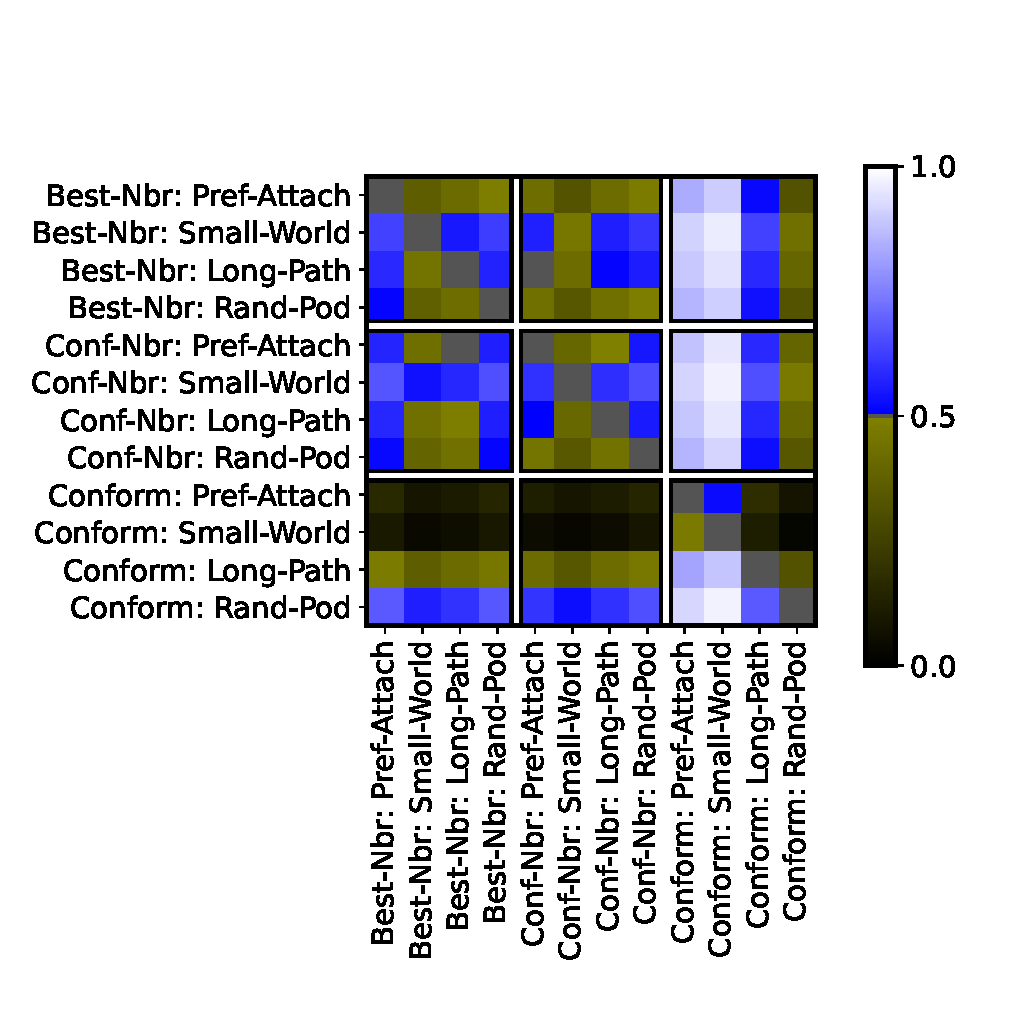
\includegraphics[width=3.33in]{fig-result-frac-parallel.eps}
\caption{Fraction of simulations in which the row condition outperforms the column condition. Results are shown for fallback individual learning. In the case of a tie, weight is divided evenly.}
\end{figure}

\begin{figure}
    \label{fig:results-bn-parallel-dist}
    \centering
    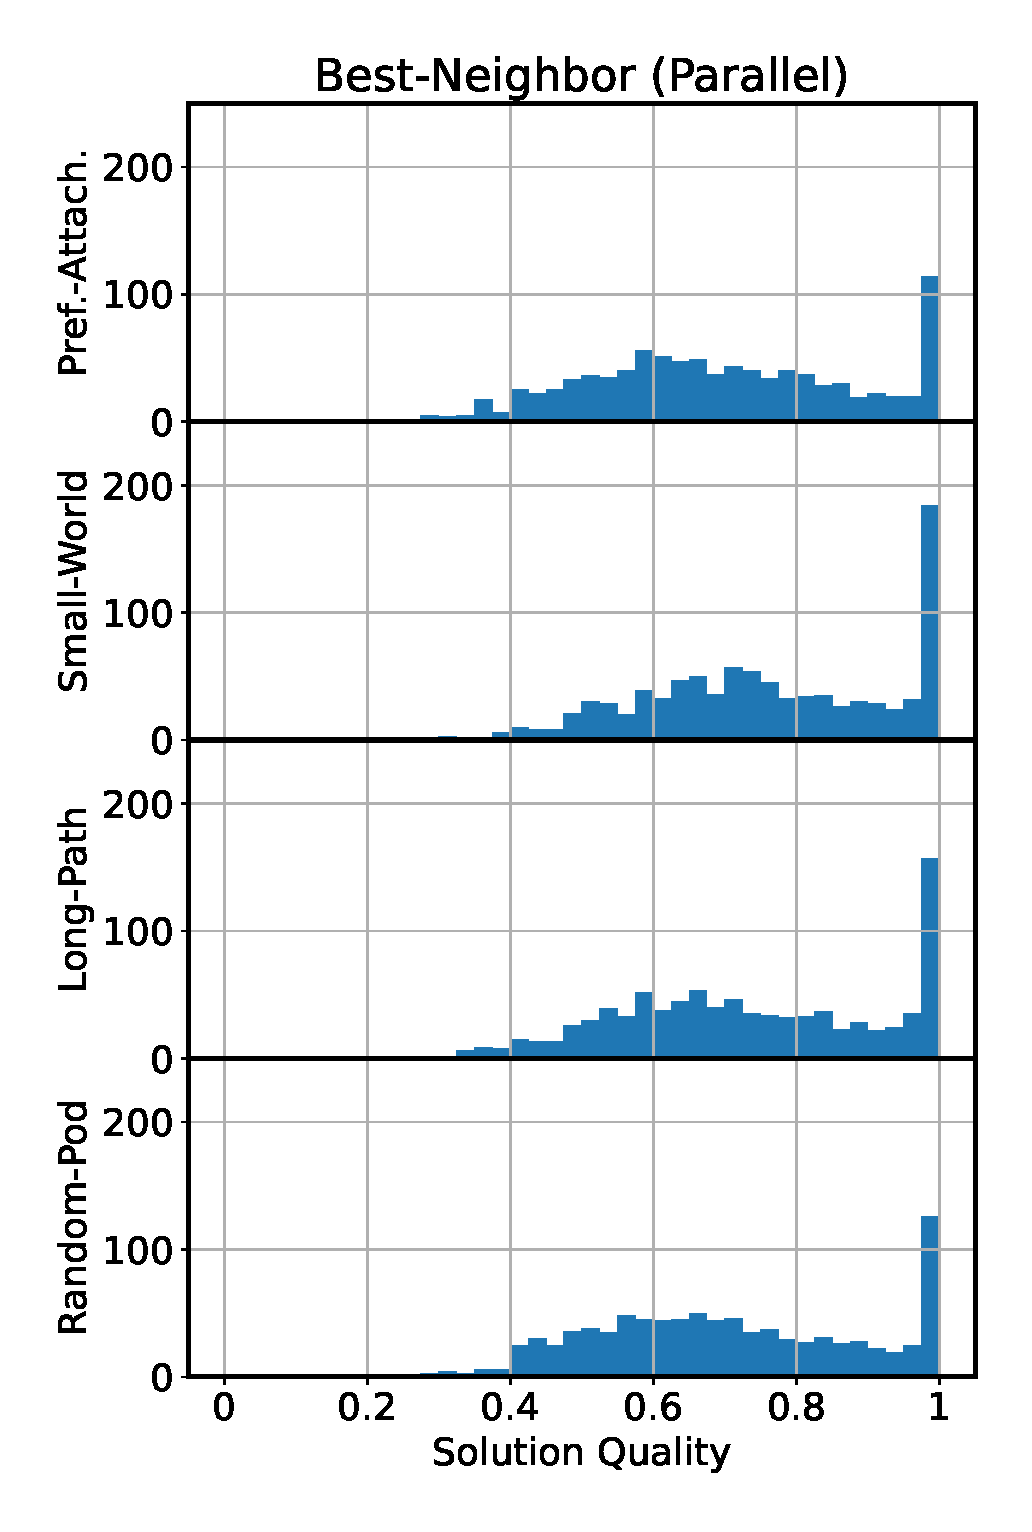
\includegraphics[width=3.33in]{results-bn-parallel-dist.eps}
\caption{Solution quality distribution for best-neighbor strategy with parallel individual learning.}
\end{figure}
\begin{figure}
    \label{fig:results-cn-parallel-dist}
    \centering
    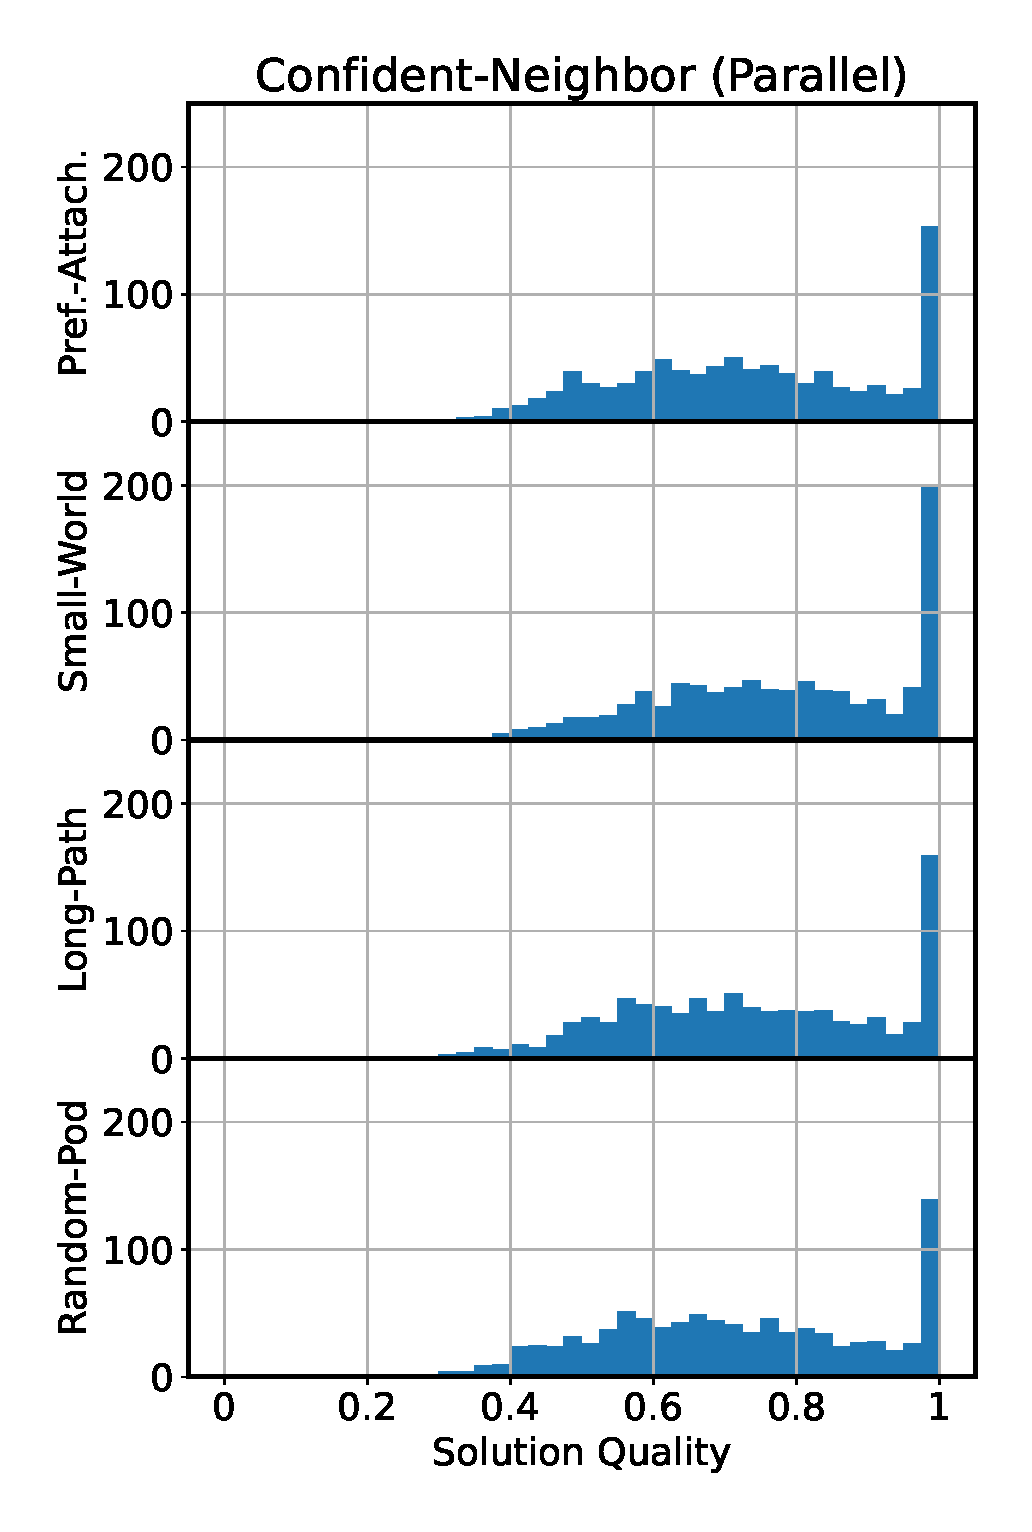
\includegraphics[width=3.33in]{results-cn-parallel-dist.eps}
\caption{Solution quality distribution for confident-neighbor strategy with parallel individual learning.}
\end{figure}
\begin{figure}
    \label{fig:results-conf-parallel-dist}
    \centering
    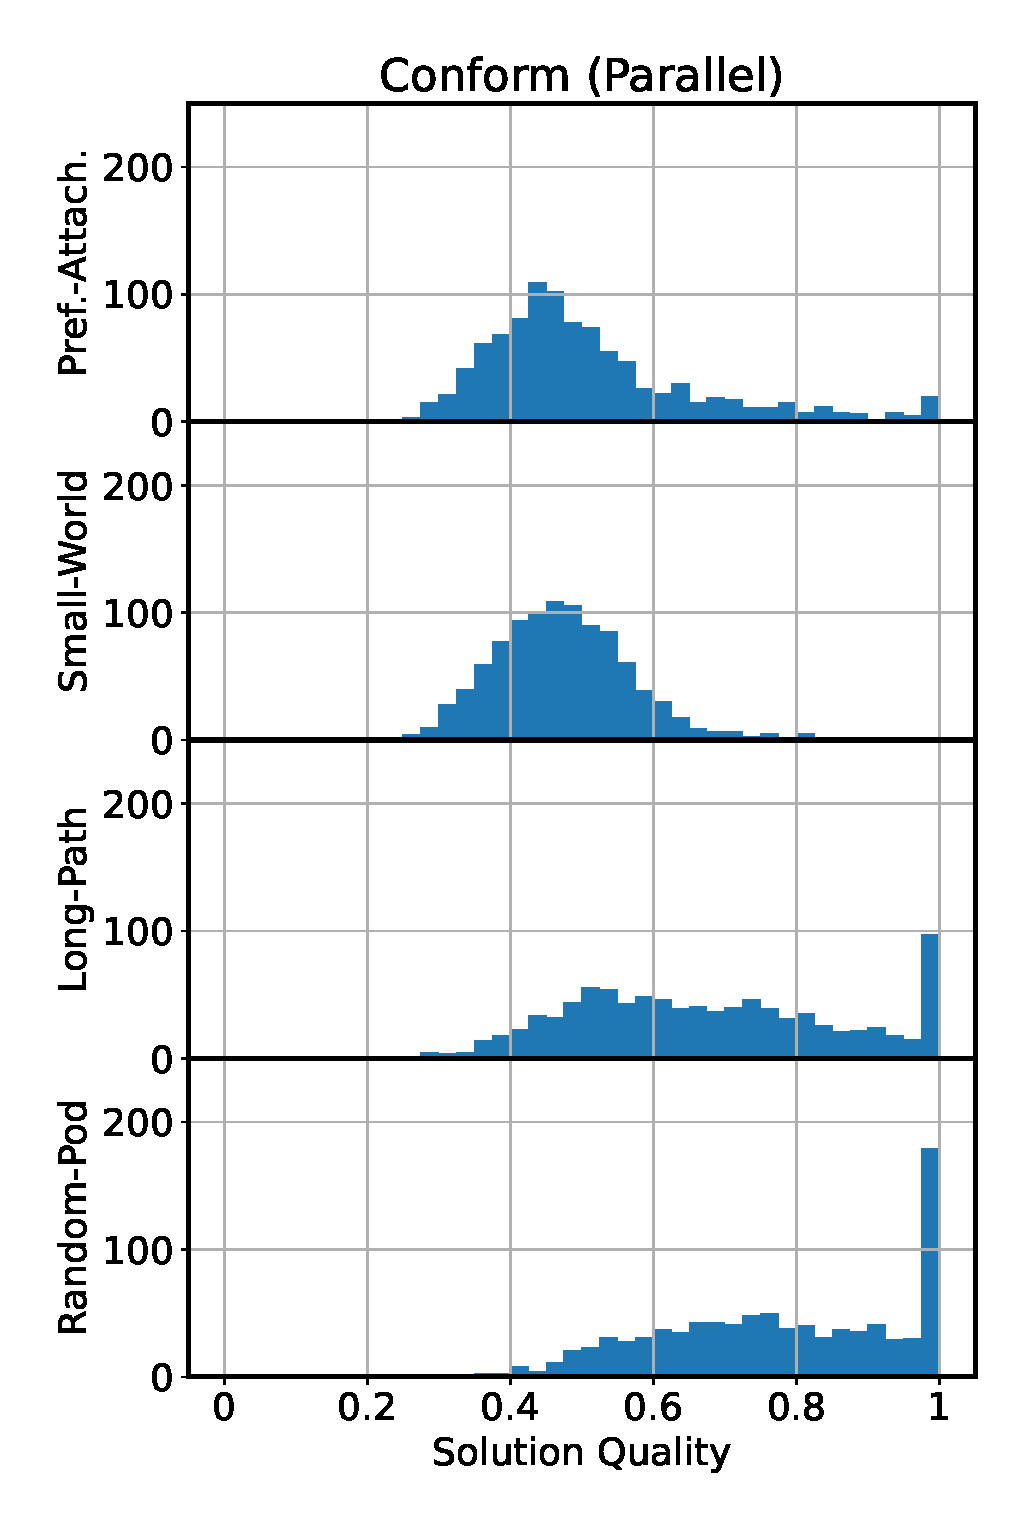
\includegraphics[width=3.33in]{results-conf-parallel-dist.eps}
\caption{Solution quality distribution for the conform strategy with parallel individual learning.}
\end{figure}

\begin{figure}
    \label{fig:results-bn-fallback-dist}
    \centering
    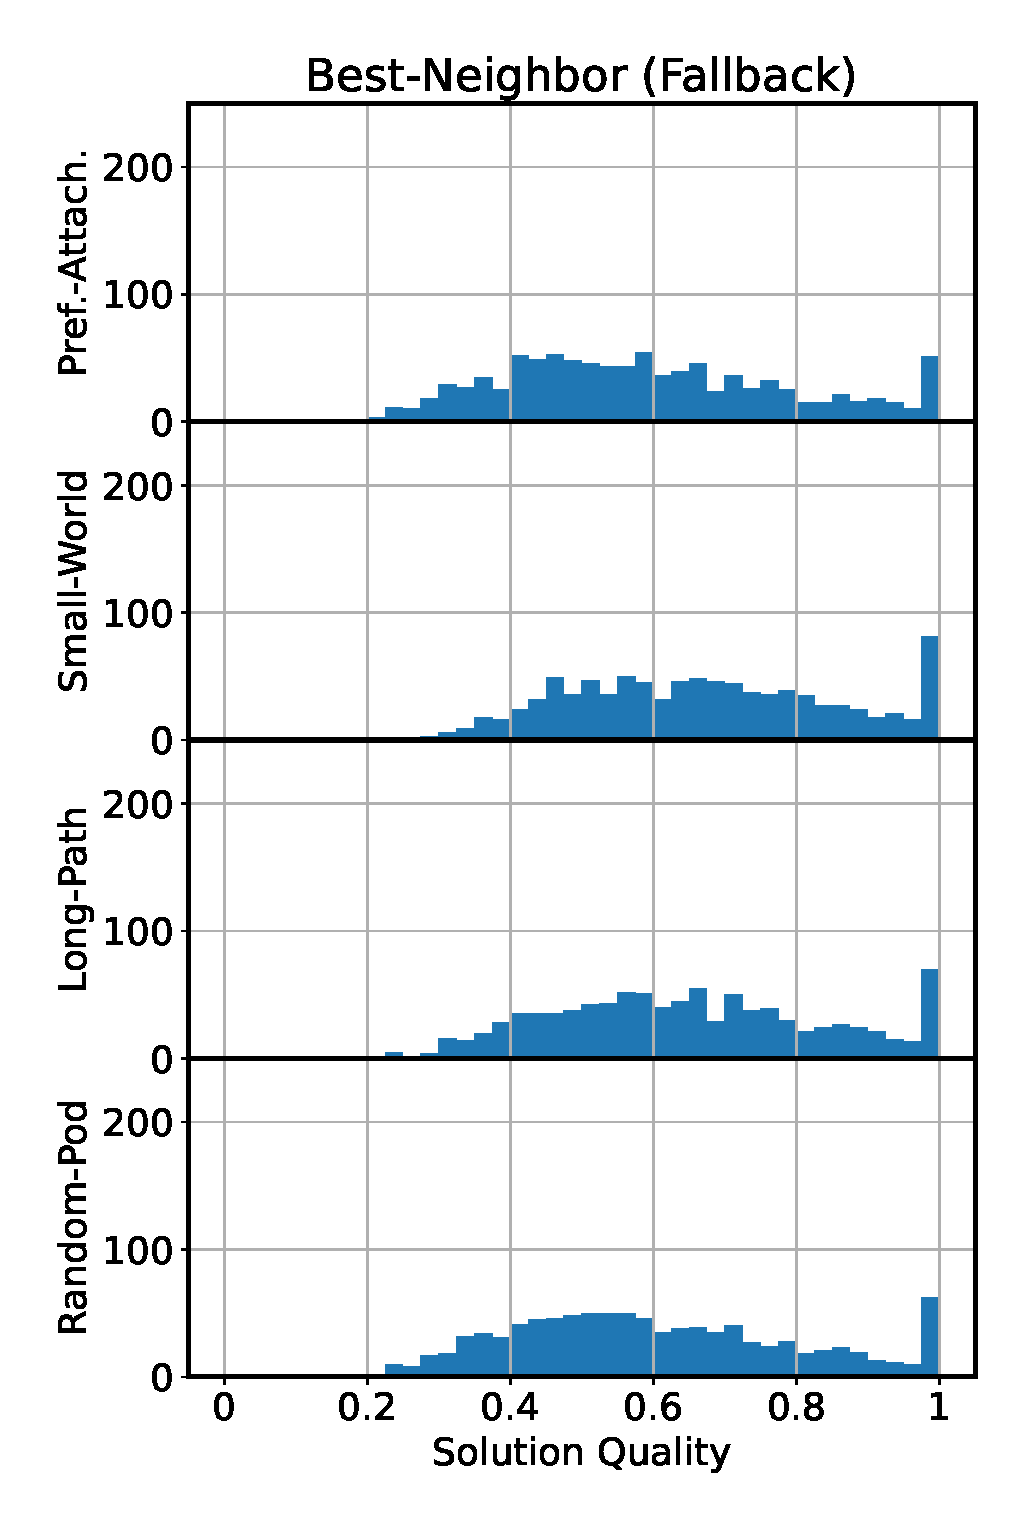
\includegraphics[width=3.33in]{results-bn-fallback-dist.eps}
\caption{Solution quality distribution for best-neighbor strategy with fallback individual learning.}
\end{figure}
\begin{figure}
    \label{fig:results-cn-fallback-dist}
    \centering
    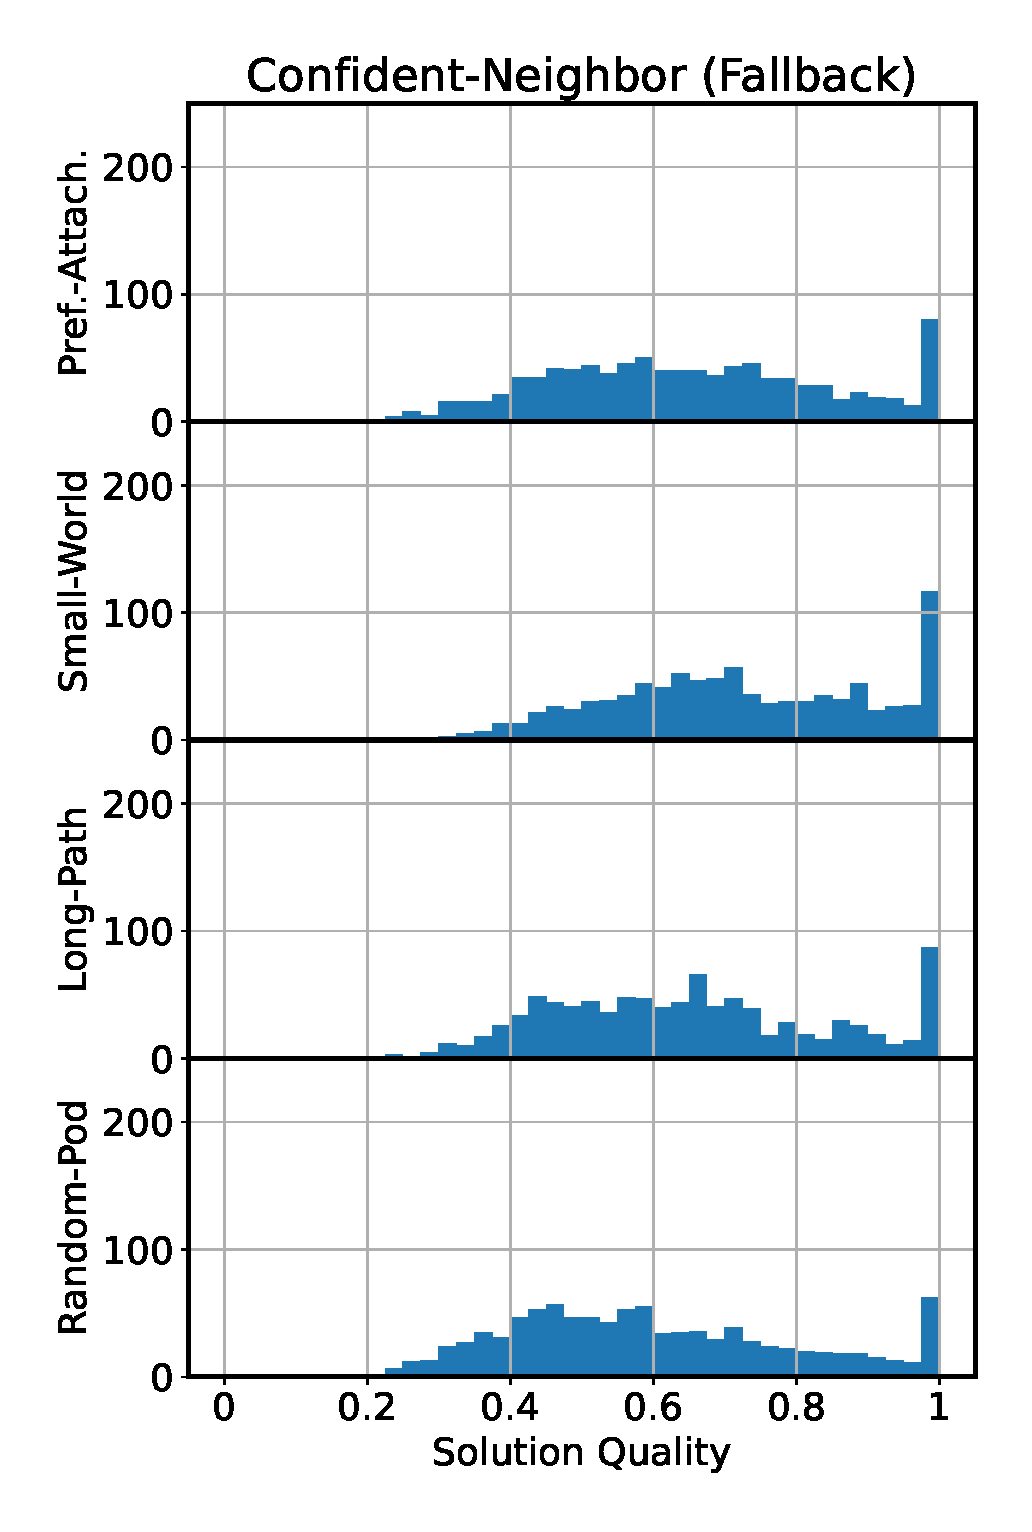
\includegraphics[width=3.33in]{results-cn-fallback-dist.eps}
\caption{Solution quality distribution for confident-neighbor strategy with fallback individual learning.}
\end{figure}
\begin{figure}
    \label{fig:results-conf-fallback-dist}
    \centering
    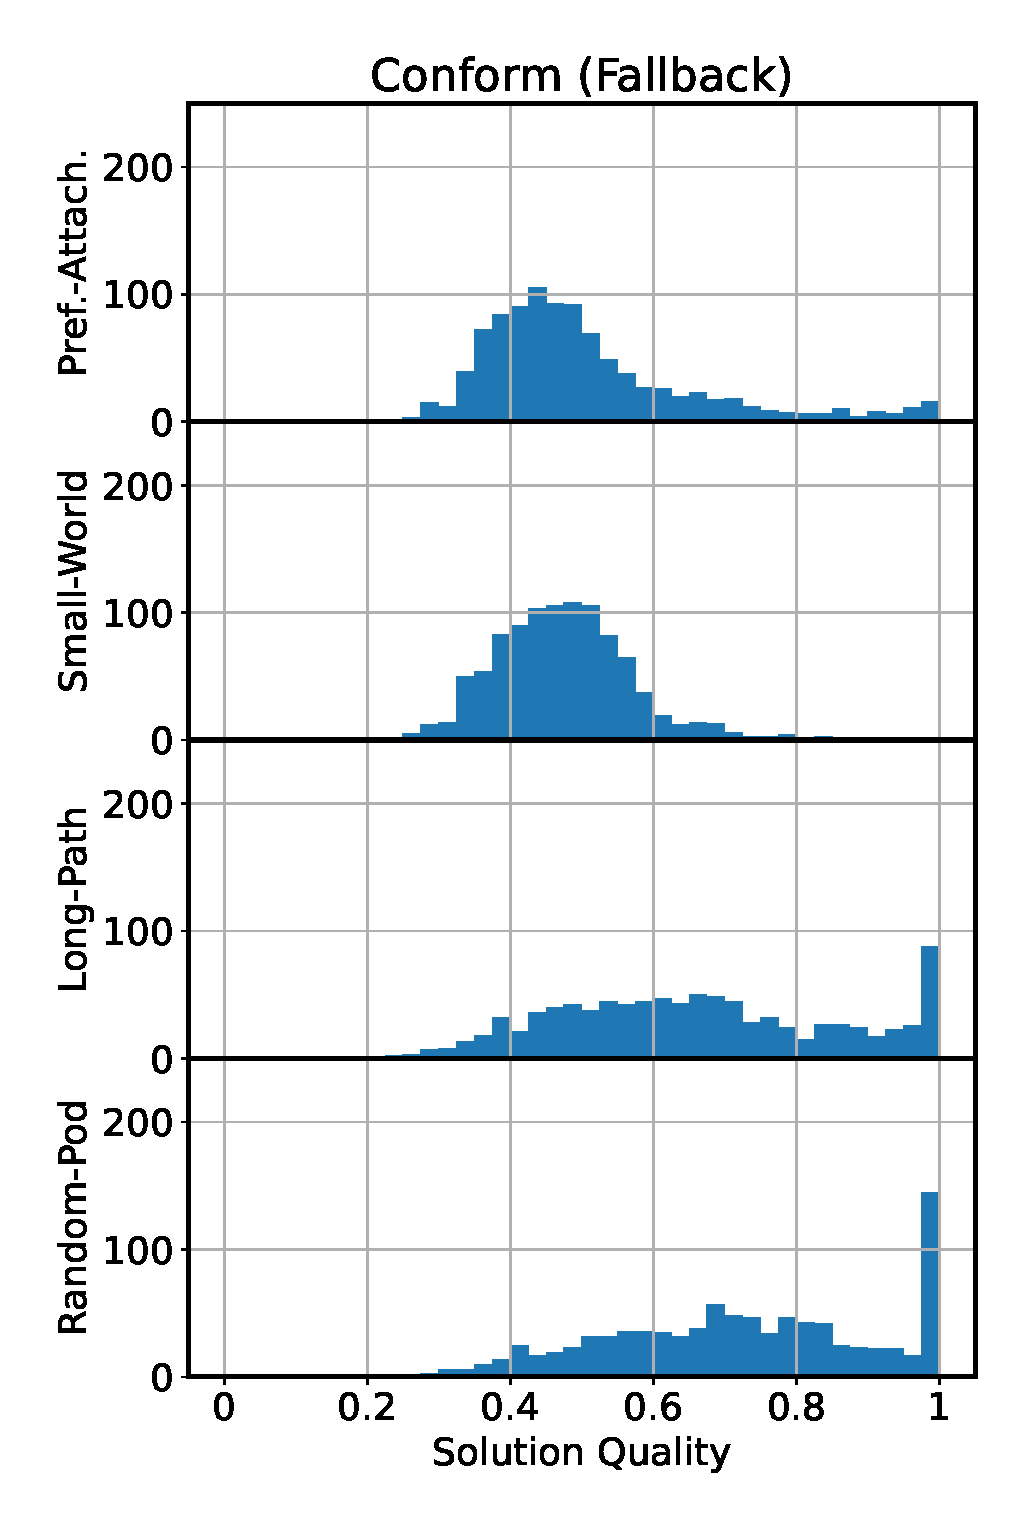
\includegraphics[width=3.33in]{results-conf-fallback-dist.eps}
\caption{Solution quality distribution for the conform strategy with fallback individual learning.}
\end{figure}

\begin{table*}[]
    \label{tab:t-instrat-fallback}
    \centering
    \begin{tabular}{l|ll|ccc}
        Strategy & Net A & Net B & \overline{B - A} & t & p* \\
        \hline
Best Neighbor&Pref. Attach.&Small World&-8.70e-02&-1.33e+01&1.27e-35\\
Best Neighbor&Pref. Attach.&Long Path&-5.98e-02&-8.62e+00&1.51e-15\\
Best Neighbor&Pref. Attach.&Random Pod&-1.15e-02&-1.83e+00&4.01e+00\\
Best Neighbor&Small World&Pref. Attach.&8.70e-02&1.33e+01&1.27e-35\\
Best Neighbor&Small World&Long Path&2.72e-02&4.53e+00&3.88e-04\\
Best Neighbor&Small World&Random Pod&7.55e-02&1.18e+01&1.66e-28\\
Best Neighbor&Long Path&Pref. Attach.&5.98e-02&8.62e+00&1.51e-15\\
Best Neighbor&Long Path&Small World&-2.72e-02&-4.53e+00&3.88e-04\\
Best Neighbor&Long Path&Random Pod&4.83e-02&7.34e+00&2.69e-11\\
Best Neighbor&Random Pod&Pref. Attach.&1.15e-02&1.83e+00&4.01e+00\\
Best Neighbor&Random Pod&Small World&-7.55e-02&-1.18e+01&1.66e-28\\
Best Neighbor&Random Pod&Long Path&-4.83e-02&-7.34e+00&2.69e-11\\
\hline
Confident Neighbor&Pref. Attach.&Small World&-7.52e-02&-1.13e+01&2.94e-26\\
Confident Neighbor&Pref. Attach.&Long Path&2.39e-03&3.64e-01&4.30e+01\\
Confident Neighbor&Pref. Attach.&Random Pod&5.80e-02&8.88e+00&1.86e-16\\
Confident Neighbor&Small World&Pref. Attach.&7.52e-02&1.13e+01&2.94e-26\\
Confident Neighbor&Small World&Long Path&7.76e-02&1.21e+01&1.08e-29\\
Confident Neighbor&Small World&Random Pod&1.33e-01&1.92e+01&1.36e-68\\
Confident Neighbor&Long Path&Pref. Attach.&-2.39e-03&-3.64e-01&4.30e+01\\
Confident Neighbor&Long Path&Small World&-7.76e-02&-1.21e+01&1.08e-29\\
Confident Neighbor&Long Path&Random Pod&5.56e-02&8.50e+00&4.00e-15\\
Confident Neighbor&Random Pod&Pref. Attach.&-5.80e-02&-8.88e+00&1.86e-16\\
Confident Neighbor&Random Pod&Small World&-1.33e-01&-1.92e+01&1.36e-68\\
Confident Neighbor&Random Pod&Long Path&-5.56e-02&-8.50e+00&4.00e-15\\
\hline
Conform&Pref. Attach.&Small World&3.60e-02&6.78e+00&1.24e-09\\
Conform&Pref. Attach.&Long Path&-1.63e-01&-2.22e+01&2.25e-87\\
Conform&Pref. Attach.&Random Pod&-2.28e-01&-3.19e+01&9.08e-153\\
Conform&Small World&Pref. Attach.&-3.60e-02&-6.78e+00&1.24e-09\\
Conform&Small World&Long Path&-1.99e-01&-3.17e+01&1.59e-151\\
Conform&Small World&Random Pod&-2.64e-01&-4.43e+01&2.20e-236\\
Conform&Long Path&Pref. Attach.&1.63e-01&2.22e+01&2.25e-87\\
Conform&Long Path&Small World&1.99e-01&3.17e+01&1.59e-151\\
Conform&Long Path&Random Pod&-6.48e-02&-8.31e+00&1.79e-14\\
Conform&Random Pod&Pref. Attach.&2.28e-01&3.19e+01&9.08e-153\\
Conform&Random Pod&Small World&2.64e-01&4.43e+01&2.20e-236\\
Conform&Random Pod&Long Path&6.48e-02&8.31e+00&1.79e-14\\
\hline
    \end{tabular}
    \caption{Two-tailed paired t-values across networks, within strategies. Results are for fallback individual learning. For all rows, dof=999 and $p^*$ is the Bonferroni-corrected p-value with m=60.}
    \label{tab:my_label}
\end{table*}

\begin{table*}[]
    \label{tab:t-innet-fallback}
    \centering
    \begin{tabular}{l|ll|ccc}
        Network & Strategy A & Strategy B & \overline{B - A} & t & p* \\
        \hline
Pref. Attach.&Best Neighbor&Confident Neighbor&-6.43e-02&-9.39e+00&2.33e-18\\
Pref. Attach.&Best Neighbor&Conform&8.96e-02&1.19e+01&6.83e-29\\
Pref. Attach.&Confident Neighbor&Best Neighbor&6.43e-02&9.39e+00&2.33e-18\\
Pref. Attach.&Confident Neighbor&Conform&1.54e-01&2.06e+01&7.57e-77\\
Pref. Attach.&Conform&Best Neighbor&-8.96e-02&-1.19e+01&6.83e-29\\
Pref. Attach.&Conform&Confident Neighbor&-1.54e-01&-2.06e+01&7.57e-77\\
\hline
Small World&Best Neighbor&Confident Neighbor&-5.26e-02&-8.39e+00&9.70e-15\\
Small World&Best Neighbor&Conform&2.13e-01&3.52e+01&4.46e-175\\
Small World&Confident Neighbor&Best Neighbor&5.26e-02&8.39e+00&9.70e-15\\
Small World&Confident Neighbor&Conform&2.65e-01&4.45e+01&1.24e-237\\
Small World&Conform&Best Neighbor&-2.13e-01&-3.52e+01&4.46e-175\\
Small World&Conform&Confident Neighbor&-2.65e-01&-4.45e+01&1.24e-237\\
\hline
Long Path&Best Neighbor&Confident Neighbor&-2.12e-03&-3.42e-01&4.39e+01\\
Long Path&Best Neighbor&Conform&-1.37e-02&-1.71e+00&5.20e+00\\
Long Path&Confident Neighbor&Best Neighbor&2.12e-03&3.42e-01&4.39e+01\\
Long Path&Confident Neighbor&Conform&-1.16e-02&-1.44e+00&8.96e+00\\
Long Path&Conform&Best Neighbor&1.37e-02&1.71e+00&5.20e+00\\
Long Path&Conform&Confident Neighbor&1.16e-02&1.44e+00&8.96e+00\\
\hline
Random Pod&Best Neighbor&Confident Neighbor&5.18e-03&8.40e-01&2.41e+01\\
Random Pod&Best Neighbor&Conform&-1.27e-01&-1.64e+01&1.07e-51\\
Random Pod&Confident Neighbor&Best Neighbor&-5.18e-03&-8.40e-01&2.41e+01\\
Random Pod&Confident Neighbor&Conform&-1.32e-01&-1.67e+01&1.39e-53\\
Random Pod&Conform&Best Neighbor&1.27e-01&1.64e+01&1.07e-51\\
Random Pod&Conform&Confident Neighbor&1.32e-01&1.67e+01&1.39e-53\\
\hline
    \end{tabular}
    \caption{Two-tailed paired t-values across strategies, within networks. Results are for fallback individual learning. For all rows, dof=999 and $p^*$ is the Bonferroni-corrected p-value with m=60.}
    \label{tab:my_label}
\end{table*}

\begin{table*}[]
    \label{tab:t-instrat-parallel}
    \centering
    \begin{tabular}{l|ll|ccc}
        Strategy & Net A & Net B & \overline{B - A} & t & p* \\
    \hline
Best Neighbor&Pref. Attach.&Small World&-6.75e-02&-1.13e+01&2.48e-26\\
Best Neighbor&Pref. Attach.&Long Path&-4.24e-02&-6.78e+00&1.25e-09\\
Best Neighbor&Pref. Attach.&Random Pod&-8.14e-03&-1.32e+00&1.12e+01\\
Best Neighbor&Small World&Pref. Attach.&6.75e-02&1.13e+01&2.48e-26\\
Best Neighbor&Small World&Long Path&2.50e-02&4.25e+00&1.42e-03\\
Best Neighbor&Small World&Random Pod&5.93e-02&9.38e+00&2.54e-18\\
Best Neighbor&Long Path&Pref. Attach.&4.24e-02&6.78e+00&1.25e-09\\
Best Neighbor&Long Path&Small World&-2.50e-02&-4.25e+00&1.42e-03\\
Best Neighbor&Long Path&Random Pod&3.43e-02&5.36e+00&6.14e-06\\
Best Neighbor&Random Pod&Pref. Attach.&8.14e-03&1.32e+00&1.12e+01\\
Best Neighbor&Random Pod&Small World&-5.93e-02&-9.38e+00&2.54e-18\\
Best Neighbor&Random Pod&Long Path&-3.43e-02&-5.36e+00&6.14e-06\\
\hline
Confident Neighbor&Pref. Attach.&Small World&-4.49e-02&-7.20e+00&7.03e-11\\
Confident Neighbor&Pref. Attach.&Long Path&-5.03e-03&-7.65e-01&2.67e+01\\
Confident Neighbor&Pref. Attach.&Random Pod&2.61e-02&4.02e+00&3.74e-03\\
Confident Neighbor&Small World&Pref. Attach.&4.49e-02&7.20e+00&7.03e-11\\
Confident Neighbor&Small World&Long Path&3.99e-02&6.96e+00&3.80e-10\\
Confident Neighbor&Small World&Random Pod&7.10e-02&1.18e+01&1.98e-28\\
Confident Neighbor&Long Path&Pref. Attach.&5.03e-03&7.65e-01&2.67e+01\\
Confident Neighbor&Long Path&Small World&-3.99e-02&-6.96e+00&3.80e-10\\
Confident Neighbor&Long Path&Random Pod&3.11e-02&4.89e+00&7.03e-05\\
Confident Neighbor&Random Pod&Pref. Attach.&-2.61e-02&-4.02e+00&3.74e-03\\
Confident Neighbor&Random Pod&Small World&-7.10e-02&-1.18e+01&1.98e-28\\
Confident Neighbor&Random Pod&Long Path&-3.11e-02&-4.89e+00&7.03e-05\\
\hline
Conform&Pref. Attach.&Small World&3.67e-02&6.85e+00&7.73e-10\\
Conform&Pref. Attach.&Long Path&-1.73e-01&-2.40e+01&7.10e-99\\
Conform&Pref. Attach.&Random Pod&-2.77e-01&-4.08e+01&6.29e-213\\
Conform&Small World&Pref. Attach.&-3.67e-02&-6.85e+00&7.73e-10\\
Conform&Small World&Long Path&-2.09e-01&-3.46e+01&3.46e-171\\
Conform&Small World&Random Pod&-3.14e-01&-5.68e+01&1.63e-313\\
Conform&Long Path&Pref. Attach.&1.73e-01&2.40e+01&7.10e-99\\
Conform&Long Path&Small World&2.09e-01&3.46e+01&3.46e-171\\
Conform&Long Path&Random Pod&-1.04e-01&-1.43e+01&8.55e-41\\
Conform&Random Pod&Pref. Attach.&2.77e-01&4.08e+01&6.29e-213\\
Conform&Random Pod&Small World&3.14e-01&5.68e+01&1.63e-313\\
Conform&Random Pod&Long Path&1.04e-01&1.43e+01&8.55e-41\\
    \hline
    \end{tabular}
    \caption{Two-tailed paired t-values across networks, within strategies. Results are for parallel individual learning. For all rows, dof=999 and $p^*$ is the Bonferroni-corrected p-value with m=60.}
    \label{tab:my_label}
\end{table*}

\begin{table*}[]
    \label{tab:t-innet-parallel}
    \centering
    \begin{tabular}{l|ll|ccc}
        Network & Strategy A & Strategy B & \overline{B - A} & t & p* \\
    \hline
Pref. Attach.&Best Neighbor&Confident Neighbor&-3.78e-02&-5.94e+00&2.39e-07\\
Pref. Attach.&Best Neighbor&Conform&2.00e-01&2.77e+01&3.28e-124\\
Pref. Attach.&Confident Neighbor&Best Neighbor&3.78e-02&5.94e+00&2.39e-07\\
Pref. Attach.&Confident Neighbor&Conform&2.38e-01&3.40e+01&1.67e-167\\
Pref. Attach.&Conform&Best Neighbor&-2.00e-01&-2.77e+01&3.28e-124\\
Pref. Attach.&Conform&Confident Neighbor&-2.38e-01&-3.40e+01&1.67e-167\\
\hline
Small World&Best Neighbor&Confident Neighbor&-1.52e-02&-2.74e+00&3.80e-01\\
Small World&Best Neighbor&Conform&3.05e-01&5.30e+01&1.25e-290\\
Small World&Confident Neighbor&Best Neighbor&1.52e-02&2.74e+00&3.80e-01\\
Small World&Confident Neighbor&Conform&3.20e-01&5.89e+01&0.00e+00\\
Small World&Conform&Best Neighbor&-3.05e-01&-5.30e+01&1.25e-290\\
Small World&Conform&Confident Neighbor&-3.20e-01&-5.89e+01&0.00e+00\\
\hline
Long Path&Best Neighbor&Confident Neighbor&-3.88e-04&-6.64e-02&5.68e+01\\
Long Path&Best Neighbor&Conform&7.02e-02&9.34e+00&3.64e-18\\
Long Path&Confident Neighbor&Best Neighbor&3.88e-04&6.64e-02&5.68e+01\\
Long Path&Confident Neighbor&Conform&7.06e-02&9.15e+00&1.83e-17\\
Long Path&Conform&Best Neighbor&-7.02e-02&-9.34e+00&3.64e-18\\
Long Path&Conform&Confident Neighbor&-7.06e-02&-9.15e+00&1.83e-17\\
\hline
Random Pod&Best Neighbor&Confident Neighbor&-3.59e-03&-5.46e-01&3.51e+01\\
Random Pod&Best Neighbor&Conform&-6.84e-02&-9.54e+00&6.11e-19\\
Random Pod&Confident Neighbor&Best Neighbor&3.59e-03&5.46e-01&3.51e+01\\
Random Pod&Confident Neighbor&Conform&-6.48e-02&-8.96e+00&9.43e-17\\
Random Pod&Conform&Best Neighbor&6.84e-02&9.54e+00&6.11e-19\\
Random Pod&Conform&Confident Neighbor&6.48e-02&8.96e+00&9.43e-17\\
    \hline
    \end{tabular}
    \caption{Two-tailed paired t-values across strategies, within networks. Results are for parallel individual learning. For all rows, dof=999 and $p^*$ is the Bonferroni-corrected p-value with m=60.}
    \label{tab:my_label}
\end{table*}

\bibliography{references}
\bibliographystyle{plain}

\end{document}
